\chapter{农场}

前面我们主要围绕电路理论来讲。这一章中我们会学习如何充分利用游戏机制进行设计。在\nameref{sec22}中,我们可以学习到如何利用\nameref{app31}进行分析。

\section{彩虹砖农场}\label{sec22}
彩虹砖农场的核心思路是最大化\wiki{彩虹史莱姆}的生成率。彩虹史莱姆在\nameref{app31}中出现在\nameref{app32},优先级较低。我们需要在保留彩虹史莱姆刷怪条件的前提下尽可能阻止优先级高于彩虹史莱姆的刷怪。彩虹史莱姆刷怪要求刷怪面不低于\lstinline{worldSurface},\hyperref[app37]{神圣环境},\wiki{困难模式},\lstinline{cloudAlpha}大于\lstinline{0}。
\begin{longtable}{|c|c|}
\hline
刷怪种类&阻止方法\\\hline
\endfirsthead
\hline
刷怪种类&阻止方法\\\hline
\endhead
\hline
\endfoot
\makecell{四柱/事件/蜘蛛巢/地下沙漠/地牢/陨石/\\ 撒旦军队/霜月/南瓜月/日食/腐地蠕虫/\\ 地下蠕虫/老鼠/蜗牛/沙尘暴/附魔剑}&\makecell{容易排除,或者\\ 已经被彩虹史莱姆\\ 刷怪要求排除}\\\hline
太空&刷怪场远离太空\\\hline
昏迷男子/沉睡渔夫/受缚哥布林/受缚巫师&所有城镇NPC入住\\\hline
\makecell{巨骨舌鱼/血水母/嗜血怪/海洋/\\ 食人鱼/蓝水母/水中小动物}&避免水中刷怪\\\hline
小动物&减少生成小动物概率\\\hline
发光蘑菇地&刷怪面不能是蘑菇草皮\\\hline
宝箱怪&清除刷怪面上方的天然土墙\\\hline
幻灵/弹跳杰克南瓜灯&避开晚上\\\hline
骷髅博士/紫胶虫/困难模式丛林/丛林&刷怪面不能是丛林草皮\\\hline
丛林青蛙&避开丛林环境\\\hline
木乃伊&刷怪面不能是各种沙块\\\hline
地表神圣&\makecell{刷怪面不能是珍珠沙块、\\ 珍珠石块、神圣草皮、粉冰雪块}\\\hline
猩红之地&\makecell{刷怪面不能是猩红石块、猩红沙块、\\ 红冰雪块、猩红草皮、猩红矿}\\\hline
腐化之地&\makecell{刷怪面不能是黑檀石块、黑檀沙块、\\ 紫冰雪块、腐化草皮、魔矿}\\\hline
冰雪巨人&避开苔原环境
\end{longtable}
所以我们可以选择传送带做刷怪面,方便收集彩虹砖的同时也可以满足刷怪面的要求。

接下来尝试优化\nameref{app33}。\wiki{困难模式}中刷怪率为540,刷怪量为6。我们使用地表白天,所以跳过了第2、5、8步。我们规避了苔原环境所以跳过了第3步。第4步中,我们规避了地牢、沙尘暴、地下沙漠、丛林、陨石;神圣环境与邪恶环境不能共存,所以第4步也跳过了。第6步自然跳过。第7步暂时不考虑。使用水蜡烛和战斗药水,执行第9步得到刷怪率为202,刷怪量为18\footnote{要记住我们已经规避了太空,所以没有最后一项的计算}。

这个结果距离刷怪率极限还差很远,所以我们还要考虑增加一些环境,在可能覆盖彩虹史莱姆的刷怪和刷怪率中做取舍。

如果使用丛林环境,那么彩虹史莱姆有1/9会被青蛙取代,也就是说彩虹史莱姆的刷怪速度变为了8/9。增加了丛林环境后刷怪率为81。等效的彩虹史莱姆的刷怪率为$81/8\times 9=91.125$,好了不少。再考虑刷怪率计算的第7步,到这一步时刷怪率为216,刷怪量为9。如果可以将活跃敌怪数控制在最多3个,那么考虑到第7步,最终的刷怪率就可以到56,超过了60的极限。

综上所述,再考虑到彩虹史莱姆的生成上限(1个),我们的彩虹砖农场要求如下:
\begin{itemize}
\item 刷怪面使用传送带。
\item 使用神圣丛林环境、地表层。整个刷怪区域和刷怪面需要回避地下、太空、海洋、苔原、沙漠。
\item 需要在雨天。尽量避开晚上,如果在晚上\footnote{尤其是新月},幻灵会占用掉部分刷怪机会。
\item 使用水蜡烛和战斗药水以增加刷怪速度。
\item 需要尽快清掉刷出来的怪,整个刷怪场存活的敌怪需要控制在至多3个,以达到最大刷怪速度。
\item 远离所有城镇NPC,以阻止小动物刷怪。
\end{itemize}

\section{水晶碎块农场}
\subsection{水晶碎块的生成机制}
在\textbf{困难模式}中,游戏每一帧会将如下的步骤执行多次,执行次数=世界宽度$\times$世界高度$\times$0.000015:
\begin{enumerate}
    \item \textbf{选取支撑块。}在一个超大的矩形区域内随机取一格,如果恰好是粉冰雪块或珍珠石块,并且取的这一格在洞穴或地狱,那么有1/110的概率可以进入下一步,否则不生成水晶。这个矩形区域左右端距离世界左右端各10格,上端为地表,下端距离世界下端20格。
    \item \textbf{选取生成格。}把上一步中取到的一格叫做支撑块。在支撑块下左右三个相邻格中随机取一格,其中取下的概率是1/2,左右的概率各1/4,这一格就作为水晶的生成格。生成格不能被其他图格阻挡,否则不能生成水晶。
    \item \textbf{局部数量限制。}统计以支撑块为中心,13格$\times$13格的正方形区域内已经存在的水晶碎块数量,如果超过了1,那么不能生成水晶。
    \item \textbf{生成水晶。}如果前三步所有检查均通过,那么在生成格生成水晶。
\end{enumerate}

\subsection{三大设计要点}
一个水晶农场主要分三个部分:生长、收割、收集。在生长环节,需要选取使用粉冰雪块还是珍珠石块,还需要设计方块的摆放方式。收割可以通过简单的虚化实现,但是我们需要知道收割的频率。如果使用相对高频的驱动进行收割,那么比较消耗CPU资源;如果使用过于低频的驱动进行收割,那么容易达到局部上限。在收集环节,需要选取使用半砖、传送带还是传送机。半砖速度快,稳定性差;传送带速度慢,稳定性好;传送机速度快,稳定性快,但是不方便操作。所有这三个部分的方案设计都是通过计算实现的。

要生成水晶碎块,需要通过四层检查:选取的方块恰好可以做支撑块;1/110的概率;生成格不能被阻挡;局部数量限制。其中1/110的概率是固定值,先不管。局部数量限制是与基础生成速度相关的,如果水晶碎块生成得快,那么就很容易达到局部数量上限,否则可以忽略掉局部数量上限。

选取方块恰好可以做支撑块的概率,是矩形区域内,洞穴和地狱中粉冰雪块和珍珠石块的比例。我们先假设这个比例是100\%。生成格不能被阻挡,意味着支撑块不能过于密集,不过我们先不管,先假设这个概率也是100\%。这样的话,水晶碎块的最大生成速率是(世界宽度$\times$世界高度$\times$0.000015)个/110帧,这是整个世界中水晶碎块的速率。那么每格上水晶碎块的速率就是0.000015个/110帧\footnote{与worldSurface和rockLayer占世界高度比例相关,这里是非常粗略的估算}。13$\times$13区域的生成速率就是$0.000015\times 13^2$=0.002535个/110帧。达到局部生成上限平均需要2个/(0.002535个/110帧)=86785帧,大约是1天。

\begin{figure}
\centering
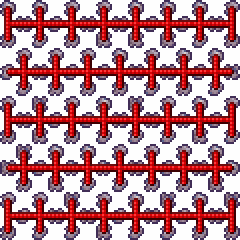
\includegraphics{images/395.png}
\caption{水晶碎块农场的最优排列与最优(?)接线。本方法的接线密度为2/3,\href{https://www.bilibili.com/video/av57287619}{沉睡的方法}的接线密度为11/16。}\label{fig28}
\end{figure}

回到前两个概率。前两个概率合起来,就是任选一个方块的一个表面,可以生成水晶的概率。换句话说,生成速率与可生成的表面积成正比。\autoref{fig28}所示的排列方式可以达到最大的表面积,在这个排列下,任选一个方块,可以做支撑块的概率是1/2,生成格不被阻挡的概率是100\%,所以水晶碎块的生成速率全部要除以2,达到局部生成上限平均需要约2天。收割周期确定为1天左右,这样不会过于频繁,也不会有太多方块达到上限。

然后考虑收割方式,是一次性虚化收割,还是一块一块收割?掉落物上限是400,一天收割一次的话,要求水晶农场的面积控制在$13\times 13\times 400\textrm{格}=67600$格以内。如果规模更大,就需要一块一块收割。这里每块的大小设置取决于收割后运输的速度。假设总共有$N$块,那么每块的收割间隔是$(86400/N)$帧。假设总面积是$S$格,那么每块的面积是$(S/N)$格,每块收割时掉落约$(S/N/169)$个水晶碎块。达到400个水晶碎块,需要收割$400/(S/N/169)=(67600N/S)$块,也就是说,水晶从掉落到收集,时间是$(86400/N)\times(67600N/S)=(5840640000/S)$帧,超过这个时间就很有可能因为掉落物上限损失水晶。对于大世界来说,$S$至多是$8400\times2400=20160000$格,时间大约是290帧,不到5秒。在5秒内收集全世界的水晶是不可能的。

水晶农场面积越小,对收集速度的要求就越低。当规模较小时,可以使用\autoref{fig28}最大化生成速率;当规模较大时,需要优先考虑便于半砖与传送器运输的结构以增加收集速度。

\section{全自动树场}
\subsection{树的生成机制}\label{sec19}
\begin{note}
本小节内容来自\href{https://github.com/sgkoishi}{sgkoishi}在\href{https://github.com/putianyi889/TerrariaWiringTutorial/pull/16}{项目PR}和\href{https://github.com/putianyi889/TerrariaWiringTutorial/issues/10#issuecomment-548415208}{项目Issues}中的贡献。
\end{note}
本小节中,“玩家附近”指玩家中心的左右0.6\lstinline{sWidth}(默认72格),上下0.6\lstinline{sHeight}(默认40.5格)范围内。\footnote{相关代码位于\lstinline{bool Terraria.WorldGen.PlayerLOS(int, int)}。}丛林红木指地表红木\footnote{地下红木只有在地图生成时才会出现,生长规律与其余地表树木类似。地下红木需要纵向12-22格的空间才会生成,高度为5-15。}。

树木生长只会发生在地图中的矩形区域内。\footnote{相关代码位于\lstinline{void Terraria.WorldGen.UpdateWorld()}。}

地表树类的矩形区域左右端和上端均距离地图边缘10格,下端为\lstinline{worldSurface}。

每次更新中,重复以下步骤($\textnormal{世界宽度}\times\textnormal{世界高度}\times 0.00003$)次:
\begin{itemize}
\item 随机选取地表矩形区域内的一个图格。
\item 如果该图格为橡树种(ID 20):
	\begin{itemize}
	\item 该格内液体量不超过32(约八分之一)。
	\item 位于玩家附近'
	\item 如果满足了本步骤中所有条件,则有1/20的几率长出树木。游戏会根据该图格的位置向下寻找最高的非橡树种方块,并将其标记为树根下方的方块。
	\end{itemize}
\item 如果该图格为丛林草地(ID 60):
	\begin{itemize}
	\item 有1/7的几率检测该图格上方有没有方块,如果没有,则长出丛林草。
	\item 如果符合以下条件,则有1/500的几率长出树木(该格视为树根下方的方块):
		\begin{itemize}
		\item 上一步中没有触发检测。
		\item 该图格上方没有方块,或只有丛林草/刺。
		\item 位于玩家附近。
		\end{itemize}
	\end{itemize}
\item 如果该格内方块类型为蘑菇草(ID 70):
	\begin{itemize}
	\item 有1/10的几率长出小蘑菇。
	\item 如果位于玩家附近,则有1/100的几率长出地表蘑菇树。
		\begin{itemize}
		\item 该格视为树根下方的方块。
		\end{itemize}
	\end{itemize}
\end{itemize}
树根下的方块上方相邻的方块标记为树根。

地下树类的矩形区域左右端均距离地图边缘10格,上端为\lstinline{worldSurface},下端为距离地图边缘20格。

每次更新中,重复以下步骤($\textnormal{世界宽度}\times\textnormal{世界高度}\times 0.000015$)次:
\begin{itemize}
\item 随机选取地下矩形区域内的一个图格。
\item 如果该格内方块类型为蘑菇草(ID 70):
	\begin{itemize}
	\item 有1/10的几率长出小蘑菇。
	\item 如果位于玩家附近,则有1/200的几率长出地下蘑菇树。
	\end{itemize}
\end{itemize}

以上提到的所有“长出树木”的过程,分为棕榈木、地下蘑菇树、其他树木。

\paragraph*{其他树木\footnote{相关代码位于\lstinline{bool Terraria.WorldGen.GrowTree(int, int)}。}}
包括普通、丛林、腐化、猩红、神圣、地表蘑菇、苔原七种树。丛林木高度上限为21,其余树木高度上限为16。

\begin{itemize}
\item 树根下方方块长有对应类型的草皮,或是雪块。
\item 树根下方的图格,其左右相邻的方块之一也符合该条件。
\item 树根所在图格完全没有液体,除非树根下的方块为丛林草地。
\item 树根所在格的背景墙为栅栏(各种木栅栏或金属栅栏),或无背景墙。
\item 树根左右2格、上方高度上限格(包括树根)的矩形区域内没有方块。
\end{itemize}
符合上述条件后,将会生成一棵树,高度为5-高度上限中的随机数值。

从树根往上,每个图格都有几率出现树枝。只有左边有、只有右边有和左右都有树枝的几率均为1/10。同一边不会出现两个上下相邻的树枝。

树根下方左右相邻的图格里,符合第一点(长草或雪地)的方块上将会长出另一块树根。

\paragraph*{棕榈木\footnote{相关代码位于\lstinline{bool Terraria.WorldGen.GrowPalmTree(int, int)}。}}
\begin{itemize}
\item 树根下方方块为沙块(普通、腐化、神圣、猩红之一)。
\item 树根所在图格没有任何液体,也没有任何背景墙。
\item 树根左右1格、上方30格(包括树根)的矩形区域内没有方块。
\end{itemize}
符合上述条件后,将会生成一棵树,高度为10-21中的随机数值。

\paragraph*{地下蘑菇树\footnote{相关代码位于\lstinline{bool Terraria.WorldGen.GrowShroom(int, int)}。}}
\begin{itemize}
\item 树根左右两格没有岩浆。
\item 树根下方左右相邻的方块均为蘑菇草地。
\item 树根左右2格,上方13格(包括树根)的矩形区域内没有方块,自然生长的蘑菇(ID 71)除外。
\end{itemize}
符合上述条件后,将会生成一棵树,高度为4-11中的随机数值。

\subsection{设计思路}
树场是相对冷门的一种农场,因为它针对的物品——木材,价值低、易获取。另一方面,一个有意义的农场至少要为玩家带来一定的便利,或者说,使用树场获取木材,需要比玩家亲手种树、亲手砍树更方便。有很多人做过所谓的树场,思路看似巧妙,但还远远不够:玩家必须亲手种树,产率低,或者收割速度不及玩家拿高阶斧子砍得快。我们不能把这些问题完全归咎于设计者,因为需要做出超过手动效率的树场不是什么易事。我们希望接下来设计的树场有如下的优势:
\begin{itemize}
\item 无需手动种树。
\item 产率高。
\item 收割速度快于斧子。
\end{itemize}

要完成“无需手动种树”的目标,我们只能选取那些可以自动生长的树种:丛林红木和蘑菇树。\nameref{sec19}告诉我们,蘑菇树的生长速度远远快于丛林红木。另一个好消息是,熔岩在流动时会烧毁周围的草皮,导致草皮上的树木崩坏;因为草皮烧毁而崩坏的树木的主干掉落的是普通的木材,而不是红木或发光蘑菇。蘑菇草皮相对于丛林草皮的另一个优势是,丛林草皮上容易长出阻止红木生成的大型丛林植物,而蘑菇草皮上的小发光蘑菇不会阻止蘑菇树生成。结论是,我们使用蘑菇草皮自动生长蘑菇树,用熔岩从下方烧毁草皮来收割树木。

影响产率的因素有:熔岩烧毁物品、凸起的图格阻止蘑菇树生成、烧毁的草皮需要重新生长。要克服这几个因素,有不少矛盾。要防止熔岩烧毁物品,就要让熔岩从下方烧毁草皮;从下方烧毁草皮,就需要用于重新扩散生长的“种子”草皮凸起在长树的平面上方;凸起的越多,草皮重新生长速度越快,而蘑菇树生成的越慢。如果我们可以定点烧毁树下的草皮,保留未长树区域的草皮,让它们扩散到被烧毁的位置,就可以规避这些矛盾。

定位树木位置相对比较简单。长了树的草皮是不能被虚化的,我们可以利用这个特性定位树木的位置。虚化所有草皮,从下往上或从上往下射飞镖,用青绿压力垫板检测飞镖是否被阻挡,就可以判断一个地方是否有树。

运输掉落的木材,可以使用传送带或半砖,我们需要根据其他设计来选用。

定点烧毁草皮较难,具体思路是这样的:只能从下方烧毁草皮,所以我们希望液体从下往上流;液体不可能从下往上流,所以必须用泵;定点烧毁,所以出水泵只能排列在草皮下方;熔岩只能烧毁周围一格的草皮,泵有两格高,所以传送的液体必须有两格高;熔岩必须停留一下才能烧毁草皮,所以出水泵必须被实体块完全包围;出水泵不能抽走液体,所以只能虚化出水泵下方的方块让熔岩流走。

三个基本的原理已经搞定,我们可以把它们组装起来了。

\subsection{实现细节}

\begin{sidewaysfigure}[p]
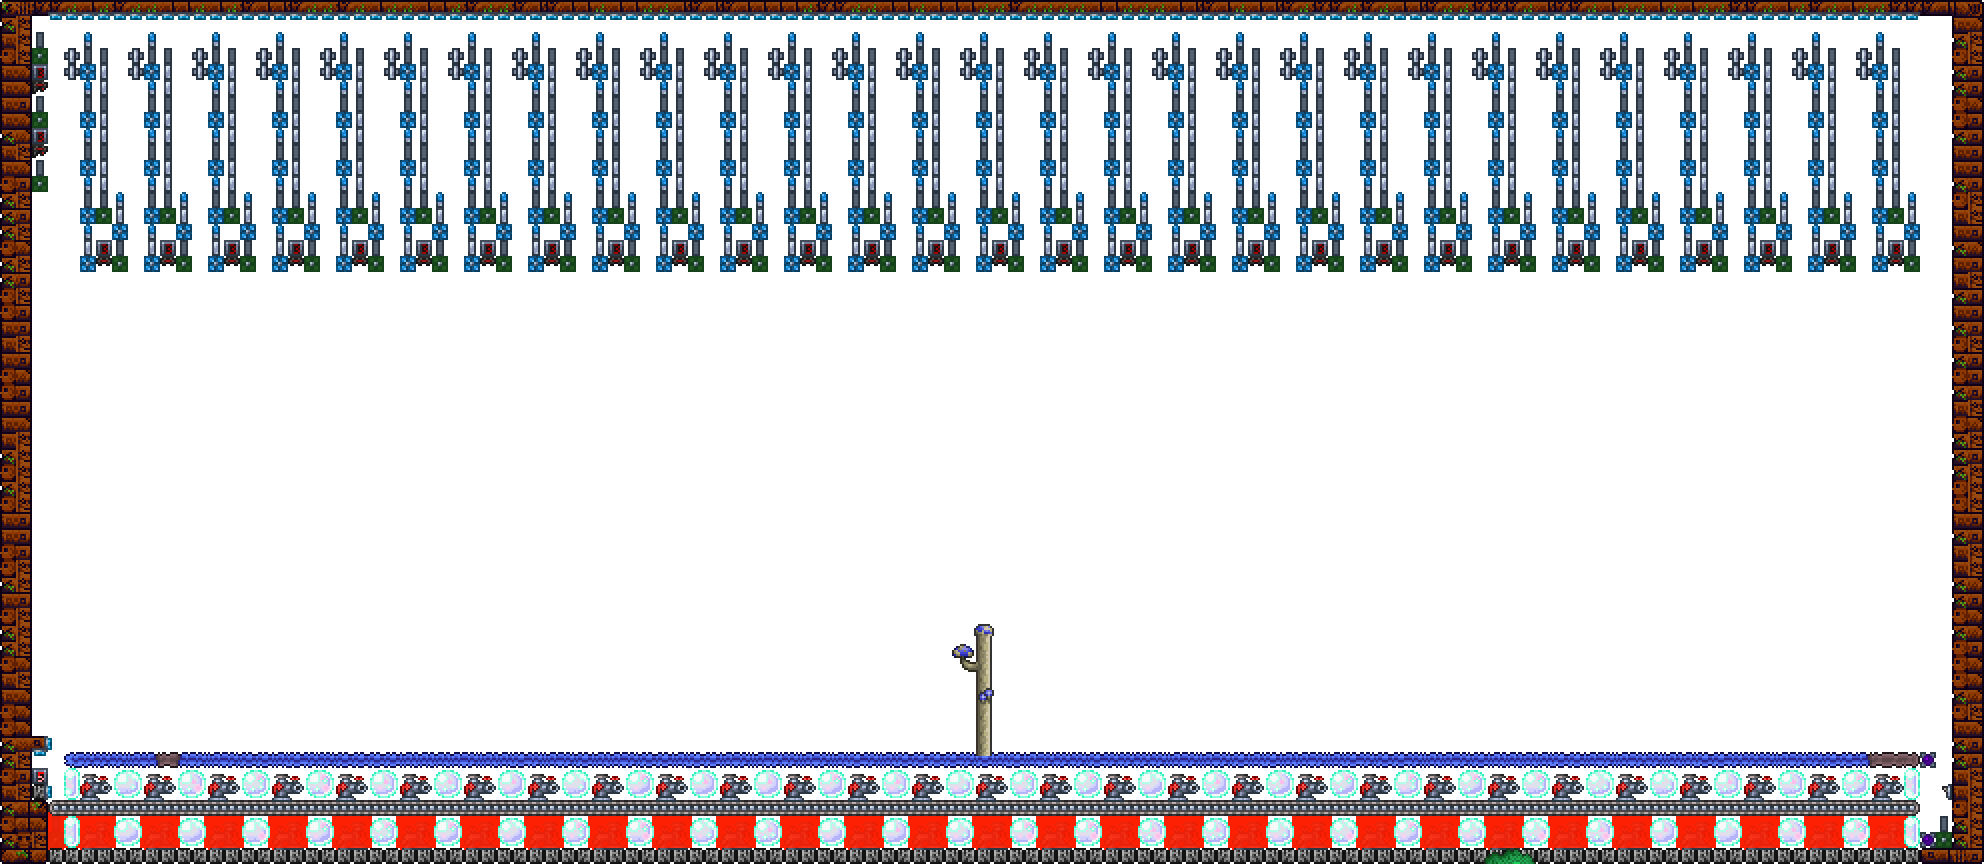
\includegraphics[width=0.99\textheight]{images/393.png}
\caption{全自动树场(隐藏电线)}\label{fig29}
\end{sidewaysfigure}

\begin{sidewaysfigure}[p]
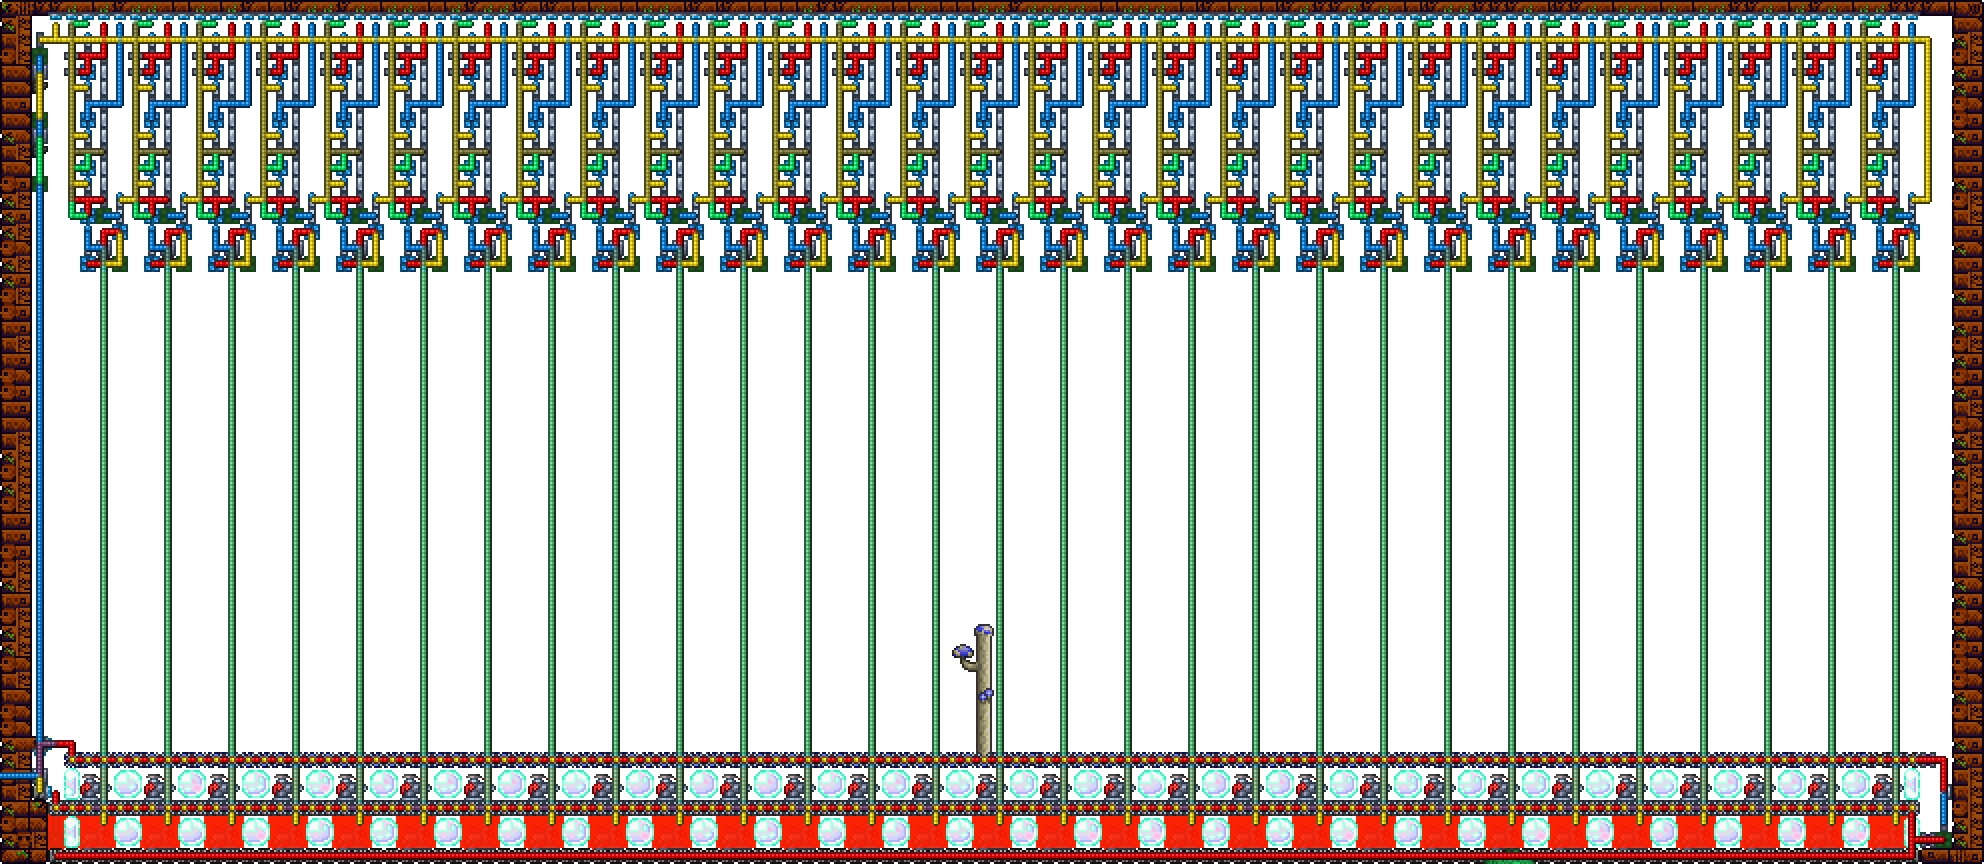
\includegraphics[width=0.99\textheight]{images/394.png}
\caption{全自动树场(显示电线)}\label{fig30}
\end{sidewaysfigure}

\autoref{fig29}和\autoref{fig30}展示了最终的全自动树场,它的工作过程如下:
\begin{enumerate}
\item 等待生长时,用5秒计时器,每5秒虚实化一次草皮,收割发光蘑菇和蘑菇草种子。这一步的本意是防止发光蘑菇阻止蘑菇树生长(当时还不知道不会阻挡),如果对发光蘑菇产量没有要求的话可以去掉。
\item 每天进行一次检测-收割操作。虚化草皮和传送带,射飞镖,飞镖通过草皮和传送带后(该时机通过对照飞镖实现)实化草皮和传送带。飞镖到达青绿压力垫板后,逻辑门发送收割信号,开始收割。
\item 接收到收割信号的收割装置,首先把熔岩泵上,烧毁草皮;然后虚化传送带,排走熔岩;然后虚化草皮,让木材掉到传送带上运走;最后复位(实化草皮)。
\end{enumerate}

设计过程考虑到了如下细节:

\begin{itemize}
\item 底端烧毁草皮装置的宽度为4,所以所有其他设计的宽度都必须小于等于4,否则摆不下(实在设计不出来的话可以考虑错位摆。很幸运的是这里设计出来了)。
\item 每次泵送熔岩至少烧毁4格草皮,所以定位树木位置时想知道是否这4格中至少有一格有树,所以用到了逻辑门。这个逻辑有3点需要注意:
	\begin{itemize}
	\item 这个逻辑的各个输入来自不同飞镖触发青绿压力垫板,所以逻辑结算是分开进行而不是统一进行,需要小心额外的激活。
	\item 有树和没有树的区别是,没有树时4个青绿压力垫板都会激活,而有树时至少有一格不激活。4个青绿压力垫板,全部接收到了信号,我们才可以确定这里没有树;而其中3个接收到信号,我们无法知道第4个是否将要接收信号。所以要设立一个对照的飞镖,如果该飞镖达到了对照的青绿压力垫板而4个青绿压力垫板中有若干仍没接收到信号,我们才可以确认这里有树。
	\item 因为逻辑结算是分开进行,所以复位也需要分开进行。这里我们利用用对照青绿压力垫板的信号复位。
	\end{itemize}
\item 对照飞镖必须比其他飞镖后达到青绿压力垫板,所以对照飞镖距离青绿压力垫板需要更远;或者在我们的实现中,将对照飞镖摆在距离电源最远的地方,让它最后被激活。需要注意的是,部分飞镖会受到熔岩减速的影响,所以对照飞镖也需要用对应格数的熔岩减速,以确保同步。
\item 泡泡可以阻挡熔岩且允许物品通过。使用其他实体块也可以,但是设计难度大幅提高\footnote{\url{https://www.bilibili.com/video/av27434278/}}。泡泡、逻辑门、传送带都是1.3.1版本更新的,没有任何理由使用逻辑门和传送带而不使用泡泡。
\item 每个收割单元使用独立的计时器,因为计时器比逻辑门占用的体积更小。
\end{itemize}

\section{生命果/世花农场}
1

\section{液体反应池}
1

\section{松露虫农场}
1

\section{采沙场}
1



\section{天梯神教}
天梯是已知最高效,并且结构相当简单的刷怪场。天梯神教的结构如\autoref{fig68}所示,由四个部分组成:天梯(蓝色)、人物活动区域(红色)、背景墙(绿色)、封刷怪(黄色)。

\begin{figure}[!ht]
\centering
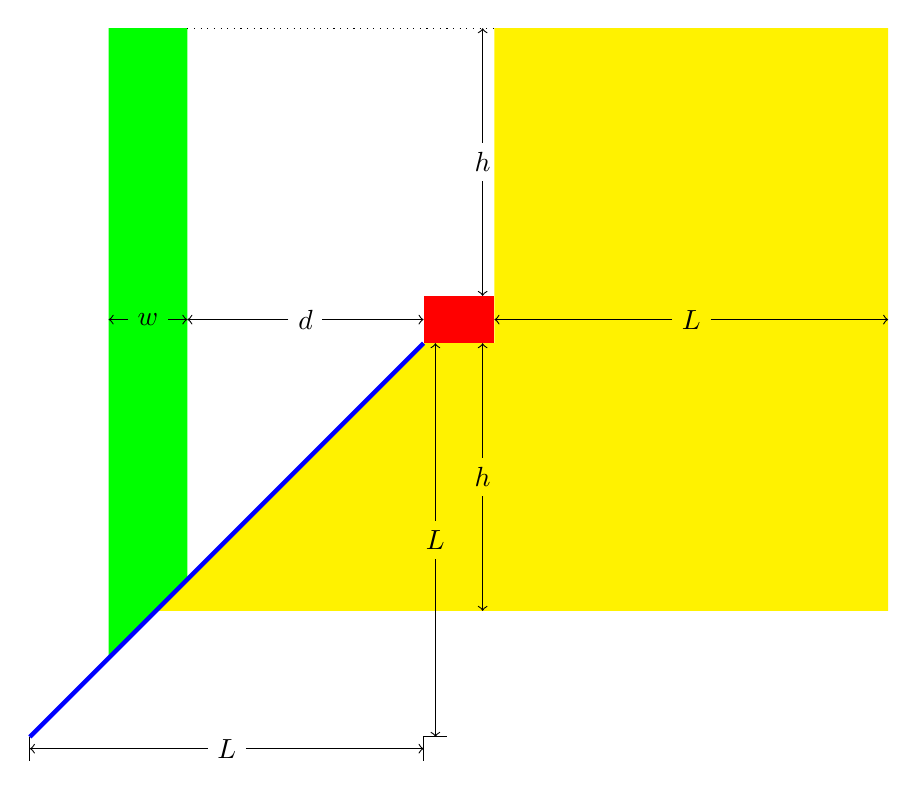
\begin{tikzpicture}
\fill[yellow] (0,0) -- (-3.4,-3.4) -- (5.9,-3.4) -- (5.9,4) -- (0.9,4) -- (0.9,0) -- (0,0);
\fill[green] (-4,-4) -- (-4,4) -- (-3,4) -- (-3,-3) -- (-4,-4);
\draw[ultra thick, blue] (-5,-5) -- (0,0);
\fill[red] (0,0) rectangle (0.9,0.6);

\draw[dotted] (-3,4) -- (0.9,4);
\node (h) at (0.75,2.3) {$h$};
\path[->] (h) edge (0.75,0.6) edge (0.75,4);
\node (h1) at (0.75,-1.7) {$h$};
\path[->] (h1) edge (0.75,0) edge (0.75,-3.4);

\node (d) at (-1.5,0.3) {$d$};
\path[->] (d) edge (-3,0.3) edge (0,0.3);
\node (w) at (-3.5,0.3) {$w$};
\path[->] (w) edge (-4,0.3) edge (-3,0.3);

\draw (0,-5.3) -- (0,-5) -- (0.3,-5);
\node (L) at (0.15,-2.5) {$L$};
\path[->] (L) edge (0.15,0) edge (0.15,-5);
\draw (-5,-5) -- (-5,-5.3);
\node (L1) at (-2.5,-5.15) {$L$};
\path[->] (L1) edge (-5,-5.15) edge (0,-5.15);
\node (L2) at (3.4,0.3) {$L$};
\path[->] (L2) edge (0.9,0.3) edge (5.9,0.3);
\end{tikzpicture}
\caption{天梯神教示意图。红色为人物活动区域及配套装置,蓝色为天梯刷怪面,绿色为人工背景墙,黄色为防止刷怪区域。}\label{fig68}
\end{figure}

天梯神教的思路是让所有敌怪刷在天梯上,然后用\wiki{终极棱镜}扫射天梯消灭所有敌怪。为了让所有敌怪刷在天梯上,天梯需要足够长,并且要对黄色区域进行封刷怪处理。所以$L$必须大于生成区域宽度\lstinline{spawnRangeX},$h$必须大于生成区域高度\lstinline{spawnRangeY}。

天梯必须是从左下到右上,而不能从右下到左上,这是因为刷怪的一个非对称机制。在\nameref{app43}中我们知道,选取刷怪面后,要判断其上6格是否有阻挡刷怪的实体块。如果天梯方向是从右下到左上,那么天梯上的图格实际上是不满足刷怪要求的(\autoref{fig71})。

\begin{figure}[!ht]
\centering
\subfloat[]{\label{fig69}
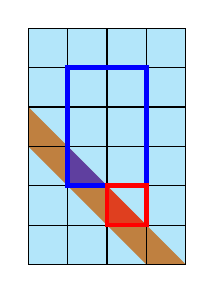
\begin{tikzpicture}
\fill[cyan!30!white] (0,1) rectangle (2,-2);
\fill[brown] (0,0) -- (2,-2) -- (1.5,-2) -- (0,-0.5);
\draw[step=0.5] (0,1) grid (2,-2);
\draw[blue,ultra thick] (0.5,0.5) rectangle (1.5,-1);
\fill[blue,opacity=0.5] (0.5,-0.5) -- (1,-1) -- (0.5,-1);
\draw[red,ultra thick] (1,-1) rectangle (1.5,-1.5);
\fill[red,opacity=0.5] (1,-1) -- (1.5,-1.5) -- (1,-1.5);
\end{tikzpicture}
}
\qquad
\subfloat[]{\label{fig70}
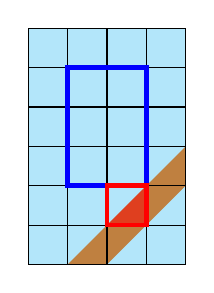
\begin{tikzpicture}
\fill[cyan!30!white] (0,1) rectangle (-2,-2);
\fill[brown] (0,-0.5) -- (-1.5,-2) -- (-1,-2) -- (0,-1);
\draw[step=0.5] (0,1) grid (-2,-2);
\draw[blue,ultra thick] (-0.5,0.5) rectangle (-1.5,-1);
\draw[red,ultra thick] (-0.5,-1) rectangle (-1,-1.5);
\fill[red,opacity=0.5] (-0.5,-1) -- (-1,-1.5) -- (-0.5,-1.5);
\end{tikzpicture}
}
\caption{\protect\subref{fig69}从右下到左上的天梯,刷怪面(红色)上方6格(蓝色)包含一个实体块(蓝色左下角),所以无法刷怪。\protect\subref{fig70}从左下到右上的天梯,刷怪面上方6格不包含实体块,可以刷怪。}\label{fig71}
\end{figure}

在\wiki{南瓜月}和\wiki{霜月}中,有些敌怪生命值与移动速度都非常高,即使使用\wiki{终极棱镜}的极限配置也可能无法在敌怪接近人物之前杀死敌怪。这时就需要防止天梯某一段的刷怪,让怪刷在远端,留出更多输出时间。影响较小的防刷怪方法是使用\hyperref[app39]{人工墙}。

为了阻止刷怪,人工墙区域顶端到人物的垂直距离显然也要大于\lstinline{spawnRangeY},所以\autoref{fig68}中把这个距离也取为$h$。

很多人可能以为$d$只要小于安全区域宽度\lstinline{safeRangeX}即可,但实际上$d$必须小于安全区域高度\lstinline{safeRangeY}。

确定人工墙区域左端的位置更困难,因为人工墙区域如果过窄,那么刷怪就可能距离人物太近,来不及杀死;人工墙区域如果过宽,就会封掉更大的生成区域,使刷怪速度降低。在这个问题上我们必须进行计算与取舍。

\begin{problem}\label{exa4}
设$\mathtt{spawnRangeX}=84$,$\mathtt{spawnRangeY}=47$,$\mathtt{safeRangeX}=62$,$\mathtt{safeRangeY}=35$,刷怪率为60,刷怪速度为$n$个/秒,固定$d=35$,求$n$与$w$的关系。
\end{problem}
\begin{solution}
实际可刷怪区域为人工墙区域左侧,天梯之上的生成区域,如\autoref{fig72}所示。

\begin{figure}[!ht]
\centering
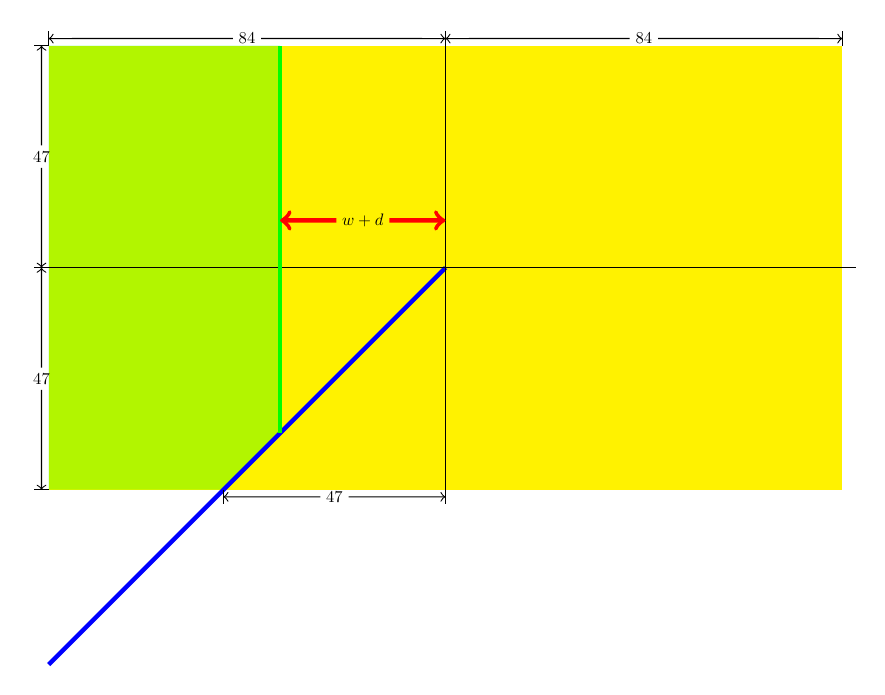
\begin{tikzpicture}[scale=0.6,transform shape]
\fill[yellow] (-8.4,4.7) rectangle (8.4,-4.7);
\fill[green,opacity=0.3] (-8.4,4.7) -- (-3.5,4.7) -- (-3.5,-3.5) -- (-4.7,-4.7) -- (-8.4,-4.7);
\draw[ultra thick, blue] (-8.4,-8.4) -- (0,0);

\draw (-8.7,0) -- (8.7,0);
\draw (0,-5) -- (0,5);
\draw (-8.7,4.7) -- (-8.4,4.7) -- (-8.4,5);
\draw (-8.7,-4.7) -- (-8.4,-4.7);
\draw (8.4,4.7) -- (8.4,5);
\draw (-4.7,-4.7) -- (-4.7,-5);

\node (a) at (-4.2,4.85) {84};
\path[->] (a) edge (-8.4,4.85) edge (0,4.85);
\node (b) at (4.2,4.85) {84};
\path[->] (b) edge (8.4,4.85) edge (0,4.85);

\node (c) at (-8.55,2.35) {47};
\path[->] (c) edge (-8.55,4.7) edge (-8.55,0);
\node (d) at (-8.55,-2.35) {47};
\path[->] (d) edge (-8.55,-4.7) edge (-8.55,0);

\node (e) at (-2.35,-4.85) {47};
\path[->] (e) edge (-4.7,-4.85) edge (0,-4.85);

\draw[green,ultra thick] (-3.5,-3.5) -- (-3.5,4.7);

\node (f) at (-1.75,1) {$w+d$};
\path[->,red,ultra thick] (f) edge (-3.5,1) edge (0,1);
\end{tikzpicture}
\caption{中央横线和中央竖线自带一格宽度,黄色区域是宽169格,高95格的生成区域。人工墙区域左侧,天梯之上的生成区域以绿色标记。}\label{fig72}
\end{figure}

设该区域的面积为$S$格,则
\begin{equation}\label{eq1}
S=
\begin{cases}{}
95(49-w), & 12\le w\le 49 \\
95(49-w)-\frac{1}{2}(12-w)(13-w). & 0\le w\le 11
\end{cases}
\end{equation}

每次刷怪尝试时,在生成区域中随机选取位置,如果50次都未能选取到可刷怪区域则刷怪失败。所以刷怪失败的概率$P$为
\begin{equation}\label{eq2}
P=\left(1-\frac{S}{16055}\right)^{50}.
\end{equation}

刷怪率为60,意味着平均1秒1次刷怪尝试;每次刷怪尝试成功概率为$1-P$,意味着平均每秒刷$1-P$个怪,即
\begin{equation}\label{eq3}
n=1-P.
\end{equation}

\eqref{eq1}、\eqref{eq2}、\eqref{eq3}共同给出的$n$与$w$的关系如\autoref{fig73}所示。$\hfill\blacksquare$

\begin{figure}[!ht]
\centering
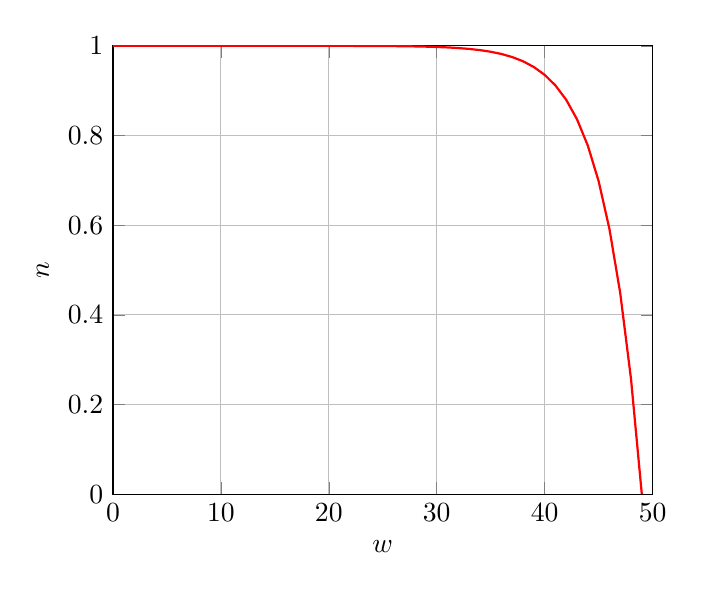
\begin{tikzpicture}
\begin{axis}[xmin=0,xmax=50,ymin=0,ymax=1,samples=50,xlabel=$w$,ylabel=$n$,grid=major]
  \addplot[red,thick,domain=0:49] {1-(1-95*(49-x)/16055)^50};
\end{axis}
\end{tikzpicture}
\caption{}\label{fig73}
\end{figure}
\end{solution}

在正常情况下,生成区域与安全区域的参数与\autoref{exa4}中的条件一样。从\autoref{fig73}中我们发现,只有当$w$非常大,使可刷怪区域宽度只有不到10格时,刷怪速度才会显著降低。对抗不同的敌怪,需要不同的天梯长度,所以人工墙具体要铺多少,留给读者思考。

配置极限伤害并不是本书关心的内容,这里略去。读者可以通过MappyGaming的演示视频学习这方面的细节:\href{https://www.bilibili.com/video/av5356226/?p=5}{南瓜月}、\href{https://www.bilibili.com/video/av5356226/?p=6}{霜月}。


\section{南瓜神教}
1

\section{全自动月亮事件}
1

\section{DPS纪录}
1

\section{速度纪录}
1

\section{Boss速杀场地}
1
